\chapter{Sub-Graph Isomorphism}
 \label{chap:subgraph}
 \hspace{10mm} In this chapter, the problem statement and various known algorithms for Sub-Graph Isomorphism are studied in great depth. 
 \section{Problem}

\fbox{
  \parbox{\textwidth}{
  \textbf{Input:} A data Graph $D$, and Query Graph $Q$. The graphs $D$ and $Q$ are undirected with nodes and edges having labels.See Figure\ref{fig:graphs}.
  \\
  Graphs given as adjacency list.\\ 
  \textbf{Output:} Give all the matching mapping of each node in $Q$ to node in $D$ \\

}
}\\\\
\begin{figure}

	\begin{minipage}{.5\textwidth}
	\centering
	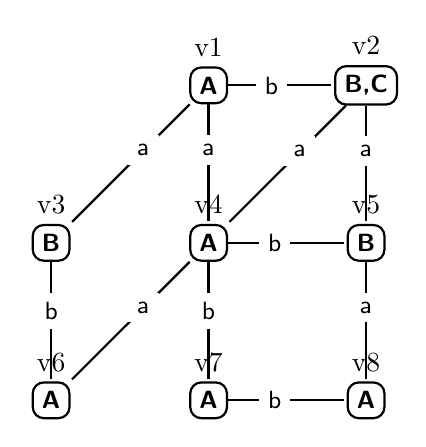
\begin{tikzpicture}[shorten >=1pt,auto,node distance=2cm,
                    thick,main node/.style={rounded corners,draw,font=\sffamily\small\bfseries}]

  \node[main node,label=v1] (1) {A};
  \node[main node,label=v2] (2) [right of=1] {B,C}; 
  \node[main node,label=v4] (4) [below of =1] {A};
  \node[main node,label=v3] (3) [left of=4] {B};
     \node[main node,label=v5] (5) [below of=2] {B};
    \node[main node,label=v6] (6) [below of=3] {A};
    \node[main node,label=v7] (7) [below of=4] {A};
\node[main node,label=v8] (8) [below of=5] {A};
  \path[every node/.style={font=\sffamily\small}]
    (1) edge[] node [minimum width = 1em, fill = white,pos=.25,right] {b} (2)
        edge[] node[minimum width = 1em, fill = white,pos=.25,below left] {a} (3)
        edge[] node[minimum width = 1em, fill = white,pos=.25,below] {a} (4)
    (2) edge[] node [minimum width = 1em, fill = white,pos=.25,below left] {a} (4)
        edge node [minimum width = 1em, fill = white,pos=.25,below] {a} (5)
    (3) edge[] node [minimum width = 1em, fill = white,pos=.25,below] {b} (6)
    (4) edge node [minimum width = 1em, fill = white,pos=.25,below] {b} (7)
    	edge[] node [minimum width = 1em, fill = white,pos=.25,below left] {a} (6) 
    	edge node [minimum width = 1em, fill = white,pos=.25,right] {b} (5) 
    (5) edge node [minimum width = 1em, fill = white,pos=.25,below] {a} (8)
    (7) edge node [minimum width = 1em, fill = white,pos=.25,right] {b} (8);	   
\end{tikzpicture}\\
Data Graph
\end{minipage}
\begin{minipage}{.5\textwidth}
\centering
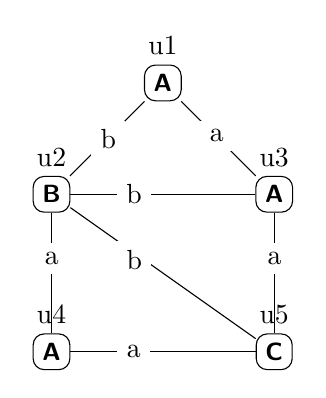
\begin{tikzpicture}[node distance=2cm,node/.style={rounded corners,draw,font=\sffamily\small\bfseries}]
	\node[node,label=u1] (1) {A};
	\node[node,label=u2] (2)[below left of=1] {B};
		\node[node,label=u3] (3)[below right of=1] {A};
		\node[node,label=u4] (4)[below  of=2] {A};
			\node[node,label=u5] (5)[below of=3] {C};
	\path
	(1) edge node [minimum width = 1em, fill = white,pos=.25,below left] {b} (2)
		edge node [minimum width = 1em, fill = white,pos=.25,below right]{a} (3)	
	(2) edge node [minimum width = 1em, fill = white,pos=.25,right]{b} (3)
		edge node [minimum width = 1em, fill = white,pos=.25,below]{a} (4)
		edge node [minimum width = 1em, fill = white,pos=.25,below right]{b} (5)
	(3) edge node [minimum width = 1em, fill = white,pos=.25,below]{a} (5)	
	(4) edge node [minimum width = 1em, fill = white,pos=.25,right]{a} (5);	
							
\end{tikzpicture}
\\ Query Graph
\end{minipage}
\caption{Data and Query Graph}
\label{fig:graphs}
\end{figure}
\hspace{10mm} In Figure \ref{fig:graphs}, 'A' and 'a' represent the node labels and edge labels. A match is present only if the edge labels and node labels are also matched. v1, v2, ... and u1, u2, ... are the node ids. They are used to explain the algorithms discussed below.
\section{Related Work}
\label{sec:rw}
\hspace{10mm}In this section we are discussing various subgraph isomorphism subgraph isomorphism algorithms. Understanding the differences in these algorithms are very crucial.
\subsection{Generic Algorithm}
\label{sec:ga}
	\hspace{10mm}The generic algorithm\cite{GEN} for subgraph isomorphism will help us to study the aspects of state-of-art algorithms in deep. It is presented in Algorithm  \ref{Graph Isomorphism}.\\
\begin{breakablealgorithm}[H]
\caption{Subgraph Search}
\label{Graph Isomorphism}
\textbf{Input}: Data Graph $D$,Query Graph $Q$.\\
\textbf{Output}: Mapping of vertices from Q to D.\\
\begin{algorithmic}
 \item \begin{enumerate}
\item for each vertex v of $Q$ 
 \begin{enumerate}
\item C(v)=$FindCandidates$(v,D)
\item If C(v) is empty return 
\end{enumerate}
\item $SUBGRAPHMATCHING$(C,Q,D,$\phi$)
\end{enumerate}
\end{algorithmic}
\textbf{Procedure $SUBGRAPHMATCHING$}:\\
\textbf{Input}: Candidates $C$,Data Graph $D$,Query Graph $Q$ Current Map $M$.\\
\textbf{Output}: Mapping of vertices from Q to D.\\
\begin{algorithmic}
\item \begin{enumerate}
\item if $|M| = |V(q)| $ report M 
\item else
 \begin{enumerate}
\item u=$NextVertex$()
\item $ C_r $ =$RefinedSet$(M,u,C(u))  
\item for each $v \in C_r$ 
 \begin{enumerate}
\item if $IsJoinable$(M,v)
 \begin{enumerate}
\item $UpdateState$(M,v)
\item $SUBGRAPHMATCHING$(q,d,C,M)
\item $RestoreState$(M,v)
\end{enumerate}
\end{enumerate}
\end{enumerate}
\end{enumerate}
\end{algorithmic}
\end{breakablealgorithm}
\hspace{10mm}The procedure $FindCandidates$ finds the vertices in datagraph which can be mapped to query vertex. The procedure $NextVertex$ finds the next vertex in querygraph which should be tried to be mapped.

\hspace{10mm}The $RefinedSet$  prunes out some nodes in the candidate set.  The $ IsJoinable$ checks whether the map is right. The $UpdateState$ moves to next state (adds new vertex to map).The $RestoreState$ removes the vertex from map and thus restores the state.

\hspace{10mm} If you consider the graphs in Figure \ref{fig:graphs}. $C(u1)=\{v1,v6,v7,v8\}$ pruned by node label and degree. Similiarly $C(u4)=\{v1,v6,v7,v8\}$ and $C(u2)=\{v3,v2,v5\}$. Procedure $NextGraph$ will give the vertices on query graph in some order like $\{u1,u2,u3,u4,u5\}$. It can be even $\{ u1, u3,u4,u2,u5\}$. Once $ u1$ is mapped to $v1$,the procedure $RefinedSet$ will remove $v1$ from $C(u4)$. If Map has these values $\{(u1,v1)\}$,$NextGraph$ returned $u2$ , $RefinedSet$ returned $\{v3,v2,v5\}$ and current $v$ is $v5$ then procedure $IsJoinable$ check whether there is an edge between $v1 $ and $v5$ like the one between $u1$ and $u2$.  
\subsection{Ullmann Algorithm}
\label{sec:ullmann}
\hspace{10mm}This algorithm\cite{Ull} is simple.The $FindCandidates$ finds same degree nodes. The $NextVertex$ takes the next node in input.The $RefinedSet$ removes nodes already mapped.  The procedure $ IsJoinable$ iterates over the neighborhood and checks if corresponding edge exists. The $UpdateState$ and $RestoreState$ adds and removes the vertex from map respectively.
\subsection{VF2 Algorithm}
\label{sec:vf2}
\hspace{10mm}VF2 algorithm was proposed in \cite{VF2}.The $NextVertex$ takes the next connected vertex. The $RefinedSet$ uses these rules
 \begin{enumerate}
 \item Prune out v if not connected from already mapped vertices.
 \item The count of unmatched vertices of neighbors of v in $Q$ must be greater than unmatched vertices of neighbors of u in $D$
 \item The count of neighbors of v who are not neighbors of mapped nodes and not mapped nodes in $Q$ must be greater than neighbors of u who are not neighbors of mapped nodes and not mapped nodes in $D$
 \end{enumerate}
\subsection{QucikSi Algorithm}
\label{sec:qsi}
\hspace{10mm}QuickSi algorithm was proposed in \cite{QSI}.The $NextVertex$ takes vertices in the most infrequent vertex first order.The $RefinedSet$ uses connectivity to mapped vertices to prune.The $RefinedSet$ only iterates over mapped adjacent vertices.
\subsection{GADDI Algorithm}
\label{sec:gaddi}
	\hspace{10mm}GADDI was proposed in \cite{GAD}. They use the neighboring discriminating substructure(NDS).$\Delta_{NDS}(u,v,P)$ is the number of occurrences of P in induced subgraph $N_k(v) \cap N_k(u)$. $N_k(u) $ is the graph having all the edges in k distance from u. A matrix L is created such that each row corresponds to an induced graph g and each column represent a pattern. See the NDS calculation in Figure \ref{fig:gaddi}. The dark lines represent the $N_k(v1) \cap N_k(v3)$ with k=2, ie., nodes and edges at a distance of at most 2 from both the vertices $v1$ and $v2$. The $NextVertex$ takes the one next in the DFS Tree from  the vertex. The $RefinedSet$ prune based on these conditions.
\\	\hspace{10mm}If for each $u^{'} \in N_{k}(u)$ there is no data vertex $v^{'} \in N_{k}(v)$ having
	\begin{enumerate}
 \item $L(u^{'}) \subseteq L(v^{'})$ 
 \item The shortest distance between $v^{'}$ and $v$ must be greater than or equal to distance between $u$ and $u^{'}$ .
 \end{enumerate}
 \begin{figure}
	\begin{minipage}{.6\textwidth}
	\centering
	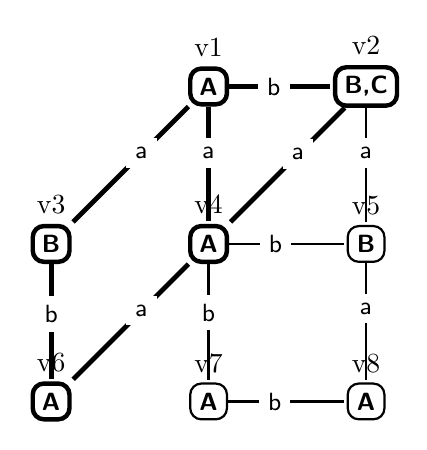
\begin{tikzpicture}[shorten >=1pt,auto,node distance=2cm,
                    thick,main node/.style={rounded corners,draw,font=\sffamily\small\bfseries}]

  \node[line width=1.6pt,main node,label=v1] (1) {A};
  \node[line width=1.6pt,main node,label=v2] (2) [right of=1] {B,C}; 
  \node[line width=1.6pt,main node,label=v4] (4) [below of =1] {A};
  \node[line width=1.6pt,main node,label=v3] (3) [left of=4] {B};
     \node[main node,label=v5] (5) [below of=2] {B};
    \node[line width=1.6pt,main node,label=v6] (6) [below of=3] {A};
    \node[main node,label=v7] (7) [below of=4] {A};
\node[main node,label=v8] (8) [below of=5] {A};
  \path[every node/.style={font=\sffamily\small}]
    (1) edge[line width=.7mm] node [minimum width = 1em, fill = white,pos=.25,right] {b} (2)
        edge[line width=.6mm] node[minimum width = 1em, fill = white,pos=.25,below left] {a} (3)
        edge[line width=.65mm] node[minimum width = 1em, fill = white,pos=.25,below] {a} (4)
    (2) edge[line width=.6mm] node [minimum width = 1em, fill = white,pos=.25,below left] {a} (4)
        edge node [minimum width = 1em, fill = white,pos=.25,below] {a} (5)
    (3) edge[line width=.65mm] node [minimum width = 1em, fill = white,pos=.25,below] {b} (6)
    (4) edge node [minimum width = 1em, fill = white,pos=.25,below] {b} (7)
    	edge[line width=.6mm] node [minimum width = 1em, fill = white,pos=.25,below left] {a} (6) 
    	edge node [minimum width = 1em, fill = white,pos=.25,right] {b} (5) 
    (5) edge node [minimum width = 1em, fill = white,pos=.25,below] {a} (8)
    (7) edge node [minimum width = 1em, fill = white,pos=.25,right] {b} (8);	   
\end{tikzpicture}\\
$ \Delta_{NDS}(v1,v3,P1)=6 , \Delta_{NDS}(v1,v3,P2)=24 ~,~\Delta_{NDS}(v1,v3,P3)=12$
\end{minipage}
\begin{minipage}{.35\textwidth}
\centering
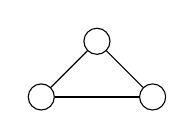
\begin{tikzpicture}[node distance=1cm]
\node[circle,draw] (1)[]{};
\node[circle,draw] (2)[below left  of=1]{};
\node[circle,draw] (3)[below right  of=1]{};
\path
	(1) edge node{} (2)
		 edge node{} (3)
	(2) edge node{} (3);	
\end{tikzpicture}
\\ P1\\ \hfill \\
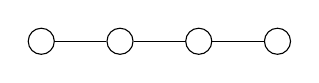
\begin{tikzpicture}[node distance=1cm]
\node[circle,draw] (1)[]{};
\node[circle,draw] (2)[right of=1]{};
\node[circle,draw] (3)[right of=2]{};
\node[circle,draw] (4)[right of=3]{};
\path
	(1) edge node{} (2)
	(2) edge node{} (3)
	(3) edge node{} (4);	
\end{tikzpicture}
\\ P2\\ \hfill \\
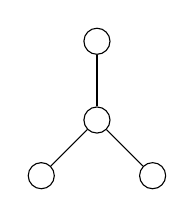
\begin{tikzpicture}[node distance=1cm]
\node[circle,draw] (4)[]{};
\node[circle,draw] (1)[below of =4]{};
\node[circle,draw] (2)[below left  of=1]{};
\node[circle,draw] (3)[below right  of=1]{};

\path
	(1) edge node{} (2)
		 edge node{} (3)
	(4) edge node{} (1);	
\end{tikzpicture}
\\ P3
\end{minipage}
\caption{GADDI NDS Calculation}
\label{fig:gaddi}
\end{figure}
\hspace{10mm}The triangles(P1) present in the $N_k(v1) \cap N_k(v3)$ is 6. The vertices $v1$, $v2$ and $v4$ make the 6 traingles(6 permutation of vertices). The number of lines of length 3(p2) present in the graph is 24. The vertices $v1$, $v2$, $v4$ and $v6$ makes one of the 24 lines. The stars(P3) present are at vertices $v1$ and $v4$. The different combinations gives 12 possibilities.
 \subsection{GraphQL Algorithm}
 \label{sec:gql}
\hspace{10mm}The GraphWl was proposed in \cite{GQL}. They use neighborhood signatures. The neighbor of the vertex is encoded as the collection of labels of its neighbors.  The $RefinedSet$  pruning is based on this signature. This is a one hop signature. For example the $sig(u1) =\{B,A\}$ in Figure \ref{fig:graphs}.

\subsection{SPath Algorithm}
\label{sec:spath}
\hspace{10mm}The SPath Algorithm was proposed in \cite{SPA}. They use signatures till k hop. They store the signature in the form $(d,l,c)$ where d is distance to the neighbor, l the label,c the  count.The $RefinedSet$  pruning is based on these signatures.For example the $sig(u1,2) = \{(1,B,1),(1,A,1),(2,A,1),(2,C,1)\}$ in Figure \ref{fig:graphs}.
\subsection{STWig Algorithm}
\label{sec:stwig}
	\hspace{10mm}The STWig Algorithm was proposed in \cite{STWig}. Here the query graph is divided into smaller graphs. These smaller graphs are searched in the data graph first. Their results are combined to get the final result. The graphs are divided such that the root of $g_j$ must be of the children of any of the graphs $g_i$ such that $i<j$. All STWigs are two level trees. See Figure \ref{fig:stwig} for a random STWigs generated for query graph in Figure \ref{fig:graphs}. There is no constraint in number of children allowed. So there are many decomposition for a graph.
	 \par The candidates can be started from the least frequent pattern and then building up. The splitting of the graphs,matching the small STWigs and then combining can be done in GPU. But the combining of STWig results in the troublesome task. This can lead to the need of large amount of memory too since the candidate set can increase exponentialy.
	\begin{figure}[h]
 \centering
%\centering
\begin{minipage}{.24\textwidth}
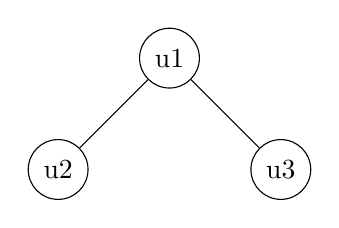
\begin{tikzpicture}[node distance=2cm]
\node[circle,draw] (1)[]{u1};
\node[circle,draw] (2)[below left  of=1]{u2};
\node[circle,draw] (3)[below right  of=1]{u3};
\path
	(1) edge node{} (2)
		 edge node{} (3);	
\end{tikzpicture}
\end{minipage}
\begin{minipage}{.24\textwidth}
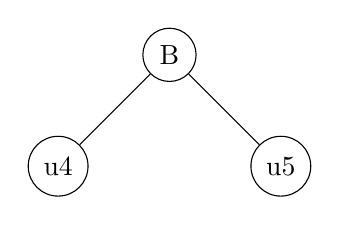
\begin{tikzpicture}[node distance=2cm]
\node[circle,draw] (1)[]{B};
\node[circle,draw] (2)[below left  of=1]{u4};
\node[circle,draw] (3)[below right  of=1]{u5};
\path
	(1) edge node{} (2)
		 edge node{} (3);	
\end{tikzpicture}
\end{minipage}
\begin{minipage}{.24\textwidth}
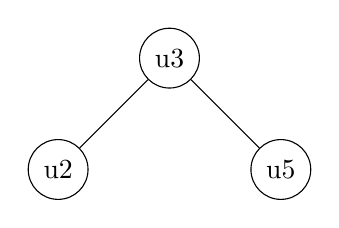
\begin{tikzpicture}[node distance=2cm]
\node[circle,draw] (1)[]{u3};
\node[circle,draw] (2)[below left  of=1]{u2};
\node[circle,draw] (3)[below right  of=1]{u5};
\path
	(1) edge node{} (2)
		 edge node{} (3);	
\end{tikzpicture}
\end{minipage}
\begin{minipage}{.24\textwidth}
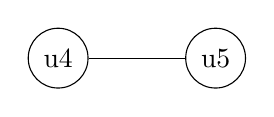
\begin{tikzpicture}[node distance=2cm]
\node[circle,draw] (1)[]{u5};
\node[circle,draw] (2)[ left  of=1]{u4};
\path
	(1) edge node{} (2)	;
\end{tikzpicture}
\end{minipage}
 \caption{STWig Decomposition}
 \label{fig:stwig}
\end{figure}
\hspace{10mm} 
\section{Implemented Algorithm}
\label{sec:implementation}
\subsection{TurboIso}
\label{sec:tiso}
	\hspace{10mm}It was proposed in \cite{Turbosio}.$Turbo_{iso}$ uses neighborhood equivalence class(NEC). Here they make a tree out of the query graph. In this tree they create the NEC. Each node will be part of a unique NEC. Later this tree is searched in the data graph. Then the graph edges are checked. 
	
	\begin{figure}[h]
 \centering
%\centering
\begin{minipage}{.6\textwidth}

\begin{tikzpicture}[node distance=2cm]
\node[circle,draw] (1)[]{5};
\node[circle,draw] (3)[below of=1]{4};
\node[circle,draw] (2)[left of=3]{2};

\node[circle,draw] (4)[ right of=3]{3};
\node[circle,draw] (5)[below of=2]{1};
\node[circle,draw] (6)[left of=5]{1};
\node[circle,draw] (7)[below of=3]{2};
\node[circle,draw] (8)[right of=7]{1};
\node[circle,draw] (9)[right of=8]{1};
\node[circle,draw] (10)[below left of=7]{1};
\node[circle,draw] (11)[below right of=7]{1};
\path
	(1) edge node{} (2)
		 edge node{} (3)
		 edge node{} (4)
	(2) edge node{} (5)
		edge node{} (6)
	(3) edge node{} (7)
		edge node{} (8)
	(4) edge node{} (9)
	(7) edge node{} (10)
		edge node{} (11);	
\end{tikzpicture}
\end{minipage}
\begin{minipage}{.2\textwidth}
\centering
NEC 4\hfill \\
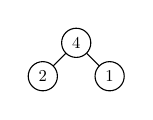
\begin{tikzpicture}[scale=0.1,every node/.style={scale=0.6}]

\node[circle,draw] (2){4};
\node[circle,draw] (3)[below left of=2]{2};
\node[circle,draw] (4)[below right of=2]{1};
\path
	(2)	 edge node{} (3)
		 edge node{} (4);
\end{tikzpicture}
\\NEC 3 \hfill \\
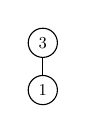
\begin{tikzpicture}[scale=0.1,every node/.style={scale=0.6}]

\node[circle,draw] (1)[]{3};
\node[circle,draw] (3)[below of=1]{1};
\path
	
	(1) edge node{} (3);
\end{tikzpicture}
\\NEC 2\hfill \\
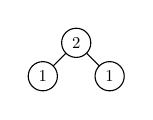
\begin{tikzpicture}[scale=0.1,every node/.style={scale=0.6}]

\node[circle,draw] (1)[]{2};
\node[circle,draw] (2)[below left of=1]{1};
\node[circle,draw] (3)[below right of=1]{1};

\path
	
	(1) edge node{} (3)
		edge node{} (2);
\end{tikzpicture}
\\NEC 5 \hfill \\
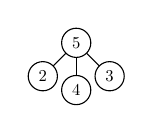
\begin{tikzpicture}[scale=0.1,every node/.style={scale=0.6}]

\node[circle,draw] (1)[]{5};
\node[circle,draw] (2)[below left of=1]{2};
\node[circle,draw] (4)[below of=1]{4};
\node[circle,draw] (3)[below right of=1]{3};

\path
	
	(1) edge node{} (3)
		edge node{} (4)
		edge node{} (2);
\end{tikzpicture}
\\Classes
\end{minipage}

 \caption{NEC Numbering}
 \label{fig:nec}
\end{figure}


\begin{algorithm}[H]

\caption{NEC creation}
%\label{Graph Isomorphism}
\textbf{Input}: Data Graph $D$,Query Graph $Q$.\\
\textbf{Output}: Mapping of vertices from Q to D.\\
\begin{algorithmic}
\item \begin{enumerate}
\item The leaf nodes are given NEC 1
\item for each level upward
\begin{enumerate}
\item Each new neighborhood will get a new NEC
\end{enumerate}
\end{enumerate}
\end{algorithmic}
\label{alg:nec}
\end{algorithm}
\hspace{10mm} In figure \ref{fig:nec}, the leaf nodes are given the NEC 1. Then the algorithm \ref{alg:nec} moves upward each level. In the succeeding level it finds two more classes NEC 2 and NEC 3. The numbering are given a sequential order. In the next level it find the NEC 5. The corresponding NEC's can be seen on the right of the image. Then CVS for each NEC is found in the data graph. Then for each combination the actual graph is tested for a match. 

\hspace{10mm} The CVS is the collection of all matching vertices of data graph for each NEC. This is found out by checking the existence of the NEC children at each data graph node. Each node in data graph is given a NEC 1. Then each higher NECs are checked. After that all possible combinations are checked for existence of the graph. If a match is found, it is printed.


\subsection{Inferences}
\label{sec:findings}
	\hspace{10mm}All of the above algorithms tried to decrease the total candidate vertices set(CVS) for a vertex in query graph. The permutation and combination of these vertices will result in the final answer. More the CVS, more will be the combinations. Since the answer requires all possible permutations we can't avoid this calculation. So we need to prune out the false candidate as early as possible. This is the reason why intermediate pruning steps are added in $UpdateState$ also. The neighborhood signature is the way seen so far to prune the CVS initially better.

